\chapter{Project Description}
Our project is an implementation of a food delivery system called MyMeal accessible as
a web page. It offers important features like 
searching for restaurants and for food available for ordering, or an ordering
process for customers. We have three kinds of user in our system: visitor, customer and restaurant.
A visitor is a person visiting our web page having no session id. A customer is already a
registered user with the possibility to order food. A restaurant is also a
registered user, who represents the restaurant with its menu.

\begin{figure}[hb]
	\centering
		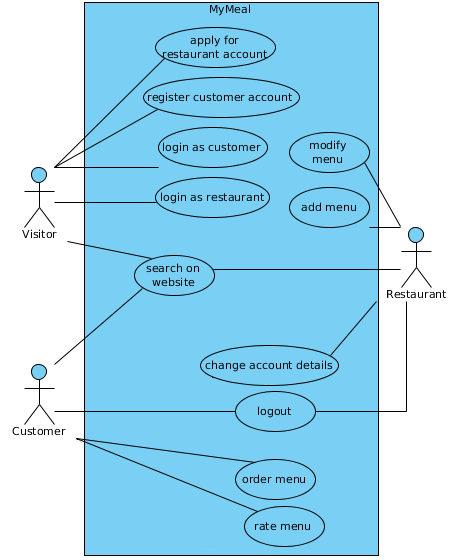
\includegraphics[scale=0.7]{content/graphics/usecase_diagram.png}
	\caption{Use case diagram of our system.}
    \label{fig:usecase_diagram}
\end{figure}


The possiblites of the users of our system are shown in figure \ref{fig:usecase_diagram}. A visitor of our website can search on it, log in as a customer or
as a restaurant, register an customer account and also apply for a restaurant account.
For now the application of a restaurant account will be processed by our similar to the
registration of a customer account. That means every restaurant will be accepted.
The application process is an optional goal.

An user logged in as a customer has the following possibilities: search
for restaurants or menus, rate a menu after it was
delivered, modify his/her rating his rating, modifying account details and
order a menu.

An user logged in as a restaurant will be able to add and modify 
his/her menus as well as the restaurant's account details 
and will also be able to search for restaurants or menus.

Optional goals: An application process for the restaurants, with 
approvement of an additional kind of user with administrative rights.
The option for a restaurant to accept or cancel an order.
The option for a customer to cancel a yet non accepted offer.
In addition we would like to offer an recommendation system for the customers based on the customer's
previous orders and ratings using machine learning techniques like neural networks
and gradient boosting.
